\documentclass[a4paper,11pt,titlepage]{article}


% -- PAQUETES -- %
\usepackage[top=1.5in, bottom=1.5in, left=1in, right=1in]{geometry}
\usepackage{amsmath,amssymb,amsfonts,latexsym,bm,mathtools,amsthm}
\usepackage{fancyhdr}
\usepackage{enumitem}
\usepackage{indentfirst}
\usepackage{subcaption}
\usepackage{graphicx}
\usepackage[utf8]{inputenc}
\usepackage{csquotes}
\usepackage{xfrac}
\usepackage{wrapfig}
\usepackage{hyperref}
\usepackage[spanish,es-tabla]{babel}
\spanishdecimal{.}
\usepackage{booktabs}
\usepackage{float}
\usepackage{longtable}
\usepackage{multirow}
\usepackage{comment}
\usepackage{svg, svgcolor}
\usepackage[backend=bibtex,style=ieee,sorting=none]{biblatex}
\addbibresource{refs.bib}
\usepackage{caption}
\usepackage{etoolbox}
\usepackage{adjustbox}
\usepackage{parskip}
\usepackage{color}
\usepackage{microtype}
\usepackage{bbm}
\usepackage[T1]{fontenc}
\usepackage{setspace}
\usepackage{ragged2e}
\usepackage{verbatim}
\usepackage{pdfpages}



% -- CUSTOM COMMANDS -- %
\newcommand{\er}[2][ecuación]{\hyperref[#2]{#1~\eqref{#2}}}
\newcommand{\nr}[2][sección]{\hyperref[#2]{#1~\ref{#2}}}
\newcommand{\n}[1]{\pmb{#1}\normalfont}
\newcommand{\crv}[1]{\emph{#1}\normalfont}
\newcommand{\uni}[1]{\pmb{\hat{#1}}}
\newcommand\YUGE{\fontsize{24.88}{40}\selectfont}
\renewcommand{\tablename}{Tabla}
\renewcommand{\numberline}[1]{#1~}
\renewcommand{\phi}{\varphi}
\DeclarePairedDelimiter\abs{\lvert}{\rvert}
\DeclarePairedDelimiter\norm{\lVert}{\rVert}
\DeclarePairedDelimiter\p{(}{)}
\DeclarePairedDelimiter\corch{[}{]}
\DeclarePairedDelimiter\brck{\{}{\}}
\DeclarePairedDelimiter\ceil{\lceil}{\rceil}
\DeclarePairedDelimiter\floor{\lfloor}{\rfloor}
\makeatletter
\let\oldabs\abs
\def\abs{\@ifstar{\oldabs}{\oldabs*}}

\let\oldnorm\norm
\def\norm{\@ifstar{\oldnorm}{\oldnorm*}}

\let\oldp\p
\def\p{\@ifstar{\oldp}{\oldp*}}

\let\oldcorch\corch
\def\corch{\@ifstar{\oldcorch}{\oldcorch*}}

\let\oldbrck\brck
\def\brck{\@ifstar{\oldbrck}{\oldbrck*}}

\let\oldceil\ceil
\def\ceil{\@ifstar{\oldceil}{\oldceil*}}

\let\oldfloor\floor
\def\floor{\@ifstar{\oldfloor}{\oldfloor*}}

\makeatother
\theoremstyle{definition}
\newtheorem{cum}{Cuestión}
\AtBeginEnvironment{proof}{\renewcommand{\qedsymbol}{}}{}{}


% -- TÍTULO SENCILLO (DESCONTINUADO) -- %
%\title{\huge{\textbf{Título Aquí}}}
%\author{Julia Gómez Concejo \and Pedro Lalanda Delgado \\[25pt] Grado en Física, 2º Curso, Grupo L13}
%\date{11 de abril, 2020}


\begin{document}


% -- LAYOUT -- %
\pagestyle{fancy}
%\nocite{*}
\fancyhf{}
\renewcommand{\headrulewidth}{2pt}
\renewcommand{\footrulewidth}{1pt}
\fancyhf[LH]{\footnotesize{\emph{Modelado tridimensional del ARN mediante Random Walks}}}
% IDs: -> Electromagnetismo: E\&M; -> ÓPTICA: OPT;
\fancyhf[RF]{\footnotesize{\thepage}}
\fancyhf[RH]{\tiny{Pedro Lalanda Delgado}}
%\renewcommand{\contentsname}{Tabla de Contenidos}
\setlength\parindent{0pt}
\setlength{\parskip}{3mm}

%\pagestyle{fancy}
%\fancyhead{}
%\fancyfoot{}
%\fancyhead[L]{\large{\sc{Visión y %telescopios}}}
%\fancyhead[R]{\slshape{Pedro L. y Julia G.}}
%\fancyfoot[C]{\thepage}


% -- TÍTULO -- %
\begin{titlepage}
\centering
{ \bfseries \Large UNIVERSIDAD COMPLUTENSE DE MADRID}
\vspace{0.5cm}

{\bfseries  \Large FACULTAD DE CIENCIAS FÍSICAS} 
\vspace{1cm}

{\large DEPARTAMENTO DE ESTRUCTURA DE LA MATERIA, FÍSICA TÉRMICA Y ELECTRÓNICA}
\vspace{0.8cm}

%%%%Logo Complutense%%%%%
{
\includegraphics[width=0.3\textwidth]{UCM.png}}

%%Para ajustar la portada a una sola página se puede reducir el tamaño del logo
\vspace{0.8cm}

%%PORTADA

{\bfseries \Large TRABAJO DE FIN DE GRADO}
\vspace{1cm}

{\Large Código de TFG:  ETE45 } \vspace{2mm}

{\Large Física Biológica}\vspace{2mm}

{\Large Biological Physics}\vspace{2mm}

{\Large Supervisor/es: Francisco J. Cao García, Juan Pedro García Villaluenga}\vspace{10mm} 

{\bfseries \LARGE Pedro Lalanda Delgado}\vspace{2mm} 

{\large Grado en Física}\vspace{2mm} 

{\large Curso acad\'emico 2023-2024}\vspace{2mm} 

{\large Convocatoria Ordinaria}\vspace{2mm} 

\end{titlepage}
\newpage

%%CONTRAPORTADA
%
%{\bfseries \large Modelado tridimensional del ARN mediante Random Walks}\vspace{10mm} 
%
%{\bfseries \large Resumen:} \vspace{5mm}
%
%Esto es una prueba para probar el formato del Resumen. Esto es una prueba para probar el formato del ResumenEsto es una prueba para probar el formato del ResumenEsto es una prueba para probar el formato del ResumenEsto es una prueba para probar el formato del ResumenEsto es una prueba para probar el formato del ResumenEsto es una prueba para probar el formato del ResumenEsto es una prueba para probar el formato del ResumenEsto es una prueba para probar el formato del ResumenEsto es una prueba para probar el formato del ResumenEsto es una prueba para probar el formato del ResumenEsto es una prueba para probar el formato del ResumenEsto es una prueba para probar el formato del ResumenEsto es una prueba para probar el formato del ResumenEsto es una prueba para probar el formato del Resumen.
%\vspace{1cm}
%
%{\bfseries \large Abstract: }\vspace{5mm} 
%
%This is a test to prove the abstract's layout.This is a test to prove the abstract's layout.This is a test to prove the abstract's layout.This is a test to prove the abstract's layout.This is a test to prove the abstract's layout.This is a test to prove the abstract's layout.This is a test to prove the abstract's layout.This is a test to prove the abstract's layout.This is a test to prove the abstract's layout.This is a test to prove the abstract's layout.This is a test to prove the abstract's layout.This is a test to prove the abstract's layout.This is a test to prove the abstract's layout.This is a test to prove the abstract's layout.This is a test to prove the abstract's layout.This is a test to prove the abstract's layout.This is a test to prove the abstract's layout.This is a test to prove the abstract's layout.This is a test to prove the abstract's layout.
%\vspace{1cm}
%
%%Comentar estas notas para que no salgan en la memoria
%{\Large\textbf{Nota: el título extendido (si procede), el resumen y el abstract deben estar en una misma página y su extensión no debe superar una página. Tamaño mínimo 11pto.}}
%\vspace{1cm}

%{\Large\textbf{Extensión máxima 20 páginas sin contar portada, contraportada y declaración responsable (sí se incluye índice, introducción, conclusiones y bibliografía}}
%\newpage

%%Incluir aquí la declaración responsable de autoría y uso de las herramientas de IA.

%{\bfseries \large INCLUIR AQUÍ la Declaración Responsable sobre Autoría y Uso Ético de Herramientas de Inteligencia Artificial}
%\vspace{1cm}
%
%El documento se puede descargar en la página web: https://fisicas.ucm.es/tfg-gradoim
%\vspace{1cm}
%
%Y en https://fisicas.ucm.es/file/declaracion-responsable-sobre-autoria-y-uso-etico-de-ia?ver
\newpage

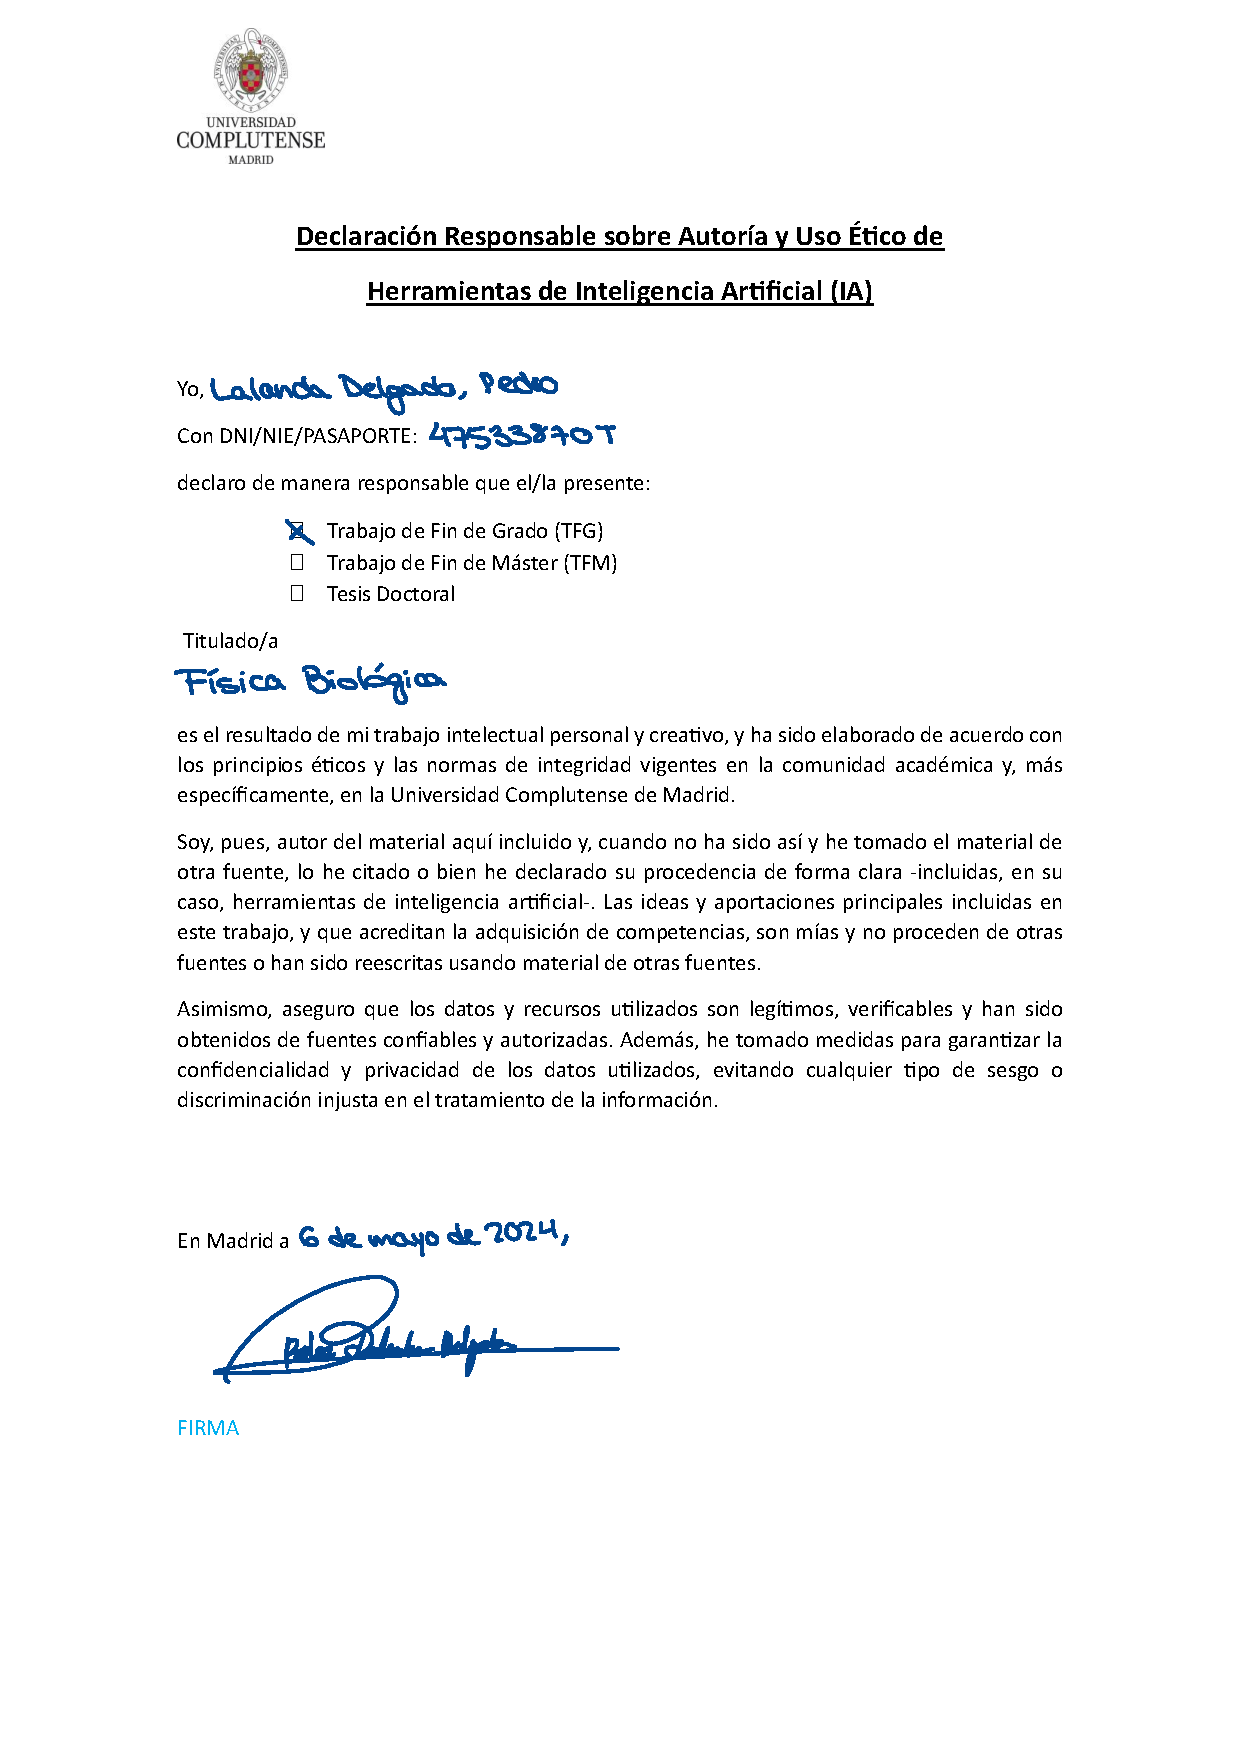
\includepdf[pages=-]{declaracion.pdf}

\newpage

\pagenumbering{arabic}
\setcounter{page}{1}
\tableofcontents

\newpage

\begin{center}
\Large\centering\textbf{Modelado tridimensional del ARN mediante Random Walks}
\end{center}

% -- ABSTRACT -- %
\section{Abstract}\label{sec:summary}

El estudio de la estructura secundaria del ARN ofrece la posibilidad de una mejor comprensión sobre los procesos biológicos de transcripción y traducción. La capacidad de predecir estructuras en base a una secuencia dada abriría la puerta a poder diseñar moléculas de ARN a nuestro interés, ya sea para modificar el comportamiento del genoma de un ser vivo, como para que cumpla una función catalítica en alguna reacción de interés. Con este objetivo, existen una serie de modelos de predicción estructural del ARN, con especial énfasis en la estructura secundaria de esta molécula. La gran mayoría de modelos tratan de predecir la estructura de ARN de menor energía libre, suponiendo que será la más probable en el equilibrio. En este trabajo, se estudia como alternativa el modelo Random Walk, una alternativa más sencilla conceptualmente, aunque en la práctica muy ineficiente. Tras comparar con el modelo ViennaRNA y con el modelo SeqFold, se ha determinado que las cadenas calculadas por Random Walks suelen no ser las más estables, y por lo tanto no se ajustan a la realidad. Se plantea como una opción posible para un estudio posterior cambiar la distribución con la que se eligen las direcciones de los segmentos, para así tener en cuenta como contribuye un segmento a la energía de conformación.

% -- INTRODUCCIÓN -- %
%\section{Introducción}\label{sec:intro}

%\newpage
% -- TEORÍA -- %
\section{Fundamento Teórico}\label{sec:thry}

\subsection{Polímeros en las Células}\label{subsec:polymers}

\begin{wrapfigure}{r}{0.5\textwidth}
    \begin{center}
      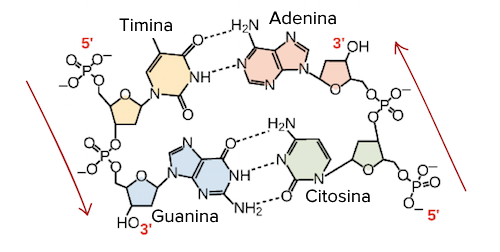
\includegraphics[width=0.35\textwidth]{adn.png}
    \end{center}
    \caption{Cadena de ADN.}
    \label{fig:adnchain}
  \end{wrapfigure}

Según el dogma central de la biología molecular, la información genética dentro de cualquier célula se transmite del ADN al ARN, por medio de la transcripción, y de este último se traduce a proteína, que es la molécula que en última instancia la célula usa para realizar una acción dada\cite{alberts}.

Por lo tanto, para el buen funcionamiento de cualquier célula viva, es necesaria la utilización de estos tres polímeros fundamentales,


\begin{enumerate}
    \item El ADN, molécula con dos cadenas en forma de doble hélice, que codifica las instrucciones genéticas necesarias para el buen funcionamiento de la maquinaria molecular de la célula. El ADN está compuesto por monómeros llamados nucleótidos, compuestos a su vez por bases nitrogenadas (A, T, C, G) complementarias dos a dos mediante enlaces de hidrógeno, y por una pentosa adherida a un grupo fosfáto. La cadenas de nucleótidos, i.e., las hélices, se mantienen unidas por enlaces covalentes entre las pentosas fosfato, y por su estructura complementaria la célula es capaz de replicar las cadenas de nucleótidos con facilidad.
    \item Las proteínas, que son las moléculas constituidas por monómeros llamados aminoácidos, que la célula usa tanto de manera estructural como para realizar una acción dada, a modo de catalizador en reacciones químicas (enzimas).
    \item El ARN, similar al ADN en su estructura en el hecho de que también esta compuesta por ácidos nucleicos (A, U, C, G), aunque en el ARN se sustituye a la timina (T) por uracilo (U). También difiere al ADN en que no suelen encontrarse dos cadenas de ARN enlazadas entre sí, encontrándose en su lugar en cadenas simples. Es interesante destacar que cada vez se descubren más casos para los que la célula utiliza el ARN, siendo también útil, por ejemplo, en reacciones catalíticas (ribozimas). En general, se clasifican las moléculas de ARN por función, por tamaño y por el lugar en el que se encuentran dentro de la célula (mRNA, tRNA, rRNA, miRNA).
\end{enumerate}


\subsection{Estructura del ARN}\label{subsec:arn}

Como he comentado previamente, en este estudio, me enfoco principalmente en la estructura que adopta la molécula de ARN, que al no estar enlazada a otra cadena complementaria, como pasa con el ADN, se dobla sobre si misma debido a la interacción que sufren entre sí los ácidos nucleicos que la componen. Cabe discutir, en este caso, la estructura que tiene el ARN y como tratar de predecir la conformación que dicha molécula va a tomar.

Cabe mencionar que la exposición teórica expuesta en esta sección se basa en el trabajo realizado por Paul G. Higgs (2000) \cite{phiggs}, quién aglutinó en la revisión citada los diferentes modelos de predicción de estructura del ARN.

El ARN esta compuesto, por cuatro ácidos nucleicos (adenina, citosina, guanina, uracilo), conectados por una cadena de ribosas, unidas entre sí por fosfatos. Es esta la principal diferencia que la estructura del ARN encuentra con la estructura del ADN, cuya cadena principal esta formada por desoxiribosas, perdiendo un átomo de oxígeno respecto a la ribosa. La otra gran diferencia que encontramos entre el ADN y el ARN es en los ácidos nucleicos que usan, principalmente en que el ADN hace uso de la timina (T) y el ARN, en cambio, hace uso del uracilo (U), aunque ambas moléculas enlazan con la adenina por medio de un enlace de hidrógeno. Cabe mencionar también que el uracilo puede enlazarse también a la guanina, cosa que con la timina no pasa y habrá que tener en cuenta más adelante.

Tanto para la cadena de ADN como para la de ARN se pueden definir direcciones en función de los átomos a los que se enlazan las ribosas y las desoxiribosas, también conocidas como pentosas. Se denomina al extremo de la cadena en la que el tercer carbono de las pentosas queda sin enlazar extremo 3' de la cadena. Por analogía, al extremo contrario, en el que el quinto carbono de las pentosas queda sin enlazar se le denomina extremo 5'.

En lo que a la estructura tridimensional que el ARN presenta, se puede estudiar en varias partes, a diferencia de las proteínas:

\begin{itemize}
    \item La estructura secundaria del ARN se refiere a los enlaces que los diferentes nucleótidos de la cadena presentan entre sí, y como esos enlaces fuerzan a la cadena a doblarse sobre sí misma. Al igual que el ADN, el ARN al doblarse sobre sí mismo forma estructuras en forma de hélice cuando dos segmentos complementarios de la cadena se enlazan. Principalmente, la estructura secundaria se describe encontrando las hélices que se forman y las secciones de nucleótidos desemparejadas que no forman hélices (hairpins, loops...).
    \item La estructura terciaria del ARN se refiere a interacciones menos relevantes entre los elementos de la cadena de ARN, como pueden ser interacciones entre tres nucleótidos, en lugar de solo dos; interacciones entre un nucleótido y la cadena de ribosas o interacciones entre secciones complementarias de nucleótidos desemparejados.
\end{itemize}

El principal objetivo de cualquier modelo computacional dedicado a predecir la estructura tridimensional del ARN es predecir correctamente su estructura secundaria, bajo la suposición de que la estructura terciaria se forma tras la conformación de la estructura secundaria, por ser interacciones con menos probabilidad de ocurrir y menos estables. A continuación expongo los diferentes modelos computacionales que existen para encontrar dicha estructura.

\subsection{Predicción de la Estructura Secundaria del ARN}\label{subsubsec:thbasis}

La mayoría de modelos computacionales tratan de encontrar la estructura del ARN que minimice la energía libre de la molécula. Para ello, se parte de unas reglas básicas: suponiendo que la cadena esta formada por $N$ nucleótidos:

\begin{itemize}
    \item Un par de bases complementarias $i$ y $j$ ha de estar al menos a cuatro nucleótidos de distancia, $\abs{i-j} \leq 4$, por ser la cadena demasiado rígida para permitir enlaces entre nucleótidos más próximos entre sí.
    \item Dadas dos parejas de bases complementarias $i-j$ y $k-l$, tomamos las parejas como compatibles, i.e., que permitimos que ambas formen parte de la estructura a predecir, sí son solapan o una esta contenida dentro de la otra ($i<j<k<l$ o $i<k<l<j$). Descartamos aquellas parejas que no cumplan estas condiciones ($i<k<j<l$, enlaces intercalados), que corresponderían a interacciones de la estructura terciaria entre segmentos lejanos de la cadena, comentados en la sección anterior.
    \item La energía libre de un nucleótido libre es mayor que la energía libre de un nucleotido enlazado. Por lo tanto, suponemos que la molécula de ARN tenderá en todo caso a doblarse sobre sí misma para enlazar la mayor cantidad de pares de nucleotidos que le sea posible.
\end{itemize}

Con estas reglas básicas se desarrollan los modelos a explicados continuación.

\subsubsection{Modelos de Programación Dinámica}\label{subsubsec:dynamic}

Los modelos más comunes con diferencia son los de programación dinámica. Estos modelos se basan en la recursión para optimizar la rapidez con la que encuentran estructuras candidatas a ser la más estable, en un tiempo que escala de acuerdo a $O(N^3)$.

El modelo más simple de esta categoría es el descrito por R. Nussinov, et. al. (1980) \cite{nussinov}. Asignamos una energía $\epsilon_{ij} = -1$ a cada par de bases enlazadas y, en caso de no estar enlazadas, asignamos una energía a la base de $\epsilon_{ij} = +\infty$, siendo $\epsilon_{ij}$ la enegía de un par de bases dado. Se pretende obtener la enegía mínima del segmento entre dos bases dadas $E_{ij}$. Supóngase que la última base, $j$, esta enlazada con una base $i < k < j$. Podemos descomponer la energía $E_{ij}$ tal que,

\begin{equation}\label{eq:recurrence}
    E_{ij} = E_{i,k-1} + E_{k+1, j-1} + \epsilon_{kj}
\end{equation}

Si la base $j$ resulta no estar enlazada con ningún nucleotido, se puede intuir de la \er[ecuación]{eq:recurrence} que $E_{ij} = E_{i,j-1}$. Partiendo de esta ecuación, se puede encontrar la energía mínima del segmento, que corresponderá con la del enlace que lo minimice, siendo esta

\begin{equation}\label{eq:mimimum}
    E_{ij} = \min\p{E_{i,j-1}, \min_{i \leq k \leq j-4}\p{E_{i,k-1} + E_{k+1, j-1} + \epsilon_{kj}}}
\end{equation}

Partiendo de la \er[ecuación]{eq:mimimum}, con un algoritmo de recursión que vaya descomponiendo el segmento a considerar en segmentos más pequeños y vaya encontrando para esos segmentos más pequeños sus energías mínimas, se puede encontrar la energía mínima de la cadena $E_{1N}$, así como la conformación de la cadena de ARN que la minimiza.

Lo que todos los modelos de programación dinámica tienen en común es el procedimiento recursivo aquí expuesto. Las diferencias entre ellos son los parámetros termodinámicos que se tienen en cuenta en los modelos, como sería en el caso del modelo expuesto $\epsilon_{ij}$. Estos parámetros se pueden ajustar para reflejar mejor los resultados obtenidos en experimentos termodinámicos realizados con cadenas de ARN. 

Cabe destacar que la energía del modelo (medida en $u.a.$ del programa), $E_{1N}$, no es la energía libre de la cadena, sino la energía total de la misma, relacionadas mediante la entropía de la cadena de acuerdo a $G = U + TS$. Lo que nos indica este hecho realmente es que a la hora de minimizar la energía libre de la cadena, hay que tener en cuenta a que temperatura a la que hacemos la aproximación. La entropía se puede calcular fácilmente partiendo de la tabla de probabilidades de cada enlace, con la expresión de la entropía de Shannon

\begin{equation}
    S_i = - \sum_{i, j} p_{ij} \log{p_{ij}}
\end{equation}

Usaré en este trabajo estos modelos como referencia para comparar los resultados obtenidos con el modelo Random Walk con los obtenidos con programación dinámica.

\subsubsection{Otros Modelos}\label{subsubsec:others}

Cabe mencionar la existencia de otros modelos de predicción de estructura del ARN, aunque no haré uso de ellos en este trabajo.

\begin{itemize}
    \item \textit{Algoritmos Kinetic Folding}: Estos modelos parten del hecho de que las energías de enlace de las hélices encontradas en el ARN suelen ser mucho mayores a la energía de las fluctuaciones térmicas, $kT$, y por lo tanto una vez formadas es extremadamente difícil que estas hélices se descompongan. Por lo tanto, se pueden encontrar las estructuras de mínima energía libre montando hélices en base a la secuencia del ARN de manera secuencial.
    \item \textit{Algoritmos Genéticos}: De la misma forma, se puede resolver el problema mediante un algoritmo que encuentre la estructura del ARN con un proceso que imite la evolución biológica: creando una población de conformaciones de cadenas heterogéneas, seleccionando las que minimicen la energía libre y mezclando su estructura para crear una nueva población (mutación y selección).
    \item \textit{Métodos Comparativos}: Es posible deducir la estructura que tomará el ARN a partir del estudio de cadenas de ARN homólogas a la estudiada en otras especies.
\end{itemize}


\subsection{Modelos Random Walk}\label{subsec:rndwalk}

Los modelos random walk son una clase de modelos basados en la idea de recorrer un espacio matemático dado mediante una sucesión de pasos tomados de manera aleatoria \cite{doyle} \cite{pearson}.

Su aplicación se extiende a múltiples disciplinas, incluyendo entre ellas a muchas originarias de la física, como pueden ser la cristalografía o la física de fluidos \cite{weiss}, así como a disciplinas ajenas al estudio del mundo natural, como puede ser el estudio de los mercados financieros\cite{blsch}.

El modelo que en este trabajo se estudia es un modelo random walk, aplicado al estudio de la estructura del ADN, conocido como el modelo freely jointed chain. En este trabajo se extiende dicho estudio al estudio del ARN. A continuación expongo el modelo freely jointed chain del ADN, que es la base de este trabajo. Se puede encontrar una explicación en detalle del modelo en R. Phillips, et. al. (2013) \cite{phillips}.

\subsubsection{Modelo Freely Jointed Chain del ADN}\label{subsubsec:rndpoly} %PAG 347

Supongamos que una cadena de ADN dada la podemos dividir en segmentos rígidos de una longitud dada, $a$, conectados entre sí por uniones flexibles. Se denomina segmentos de Kuhn a los segmentos definidos. Queremos encontrar una distribución de probabilidad $p(\vec{R}, N)$ que nos indique con que probabilidad una cadena de $N$ nucleotidos tenga uno de sus extremos situados en la posición $\vec{R}$, suponiendo que la posición del otro extremo es el origen.

Para encontrar esta distribución, vamos a limitarnos primero al caso unidimensional, $p(x, N)$. En el caso unidimensional, los segmentos consecutivos solo podrán estar dirigidos con respecto a los segmentos previos en dos direcciones: hacia la izquierda o hacia la derecha. Si asignamos la misma probabilidad de que esto ocurra a las dos direcciones, i.e., $p_l = p_r = 1/2$, podemos obtener la probabilidad de dar un total de $n_r$ pasos a la derecha del siguiente modo,

\begin{equation}\label{eq:binom}
    p\p{n_r, N} = \binom{N}{n_r} \p{\frac{1}{2}}^N = \frac{N!}{n_r! \p{N - n_r}!} \p{\frac{1}{2}}^N
\end{equation}

Podemos observar pues que la cantidad de pasos que tomo en una de las dos direcciones se ajusta a la distribución binomial. Teniendo en cuenta que $R = (n_r - n_l) a$, siendo $n_l$ el número de pasos dados a la izquierda, y que $n_r + n_l = N$, obtenemos

\begin{equation}\label{eq:fancy}
    p\p{R, N} = \frac{N!}{\p{\frac{N}{2} + \frac{R}{2a}}! \p{\frac{N}{2} - \frac{R}{2a}}!} \p{\frac{1}{2}}^N
\end{equation}

Para el caso límite en el que el tamaño de la cadena bajo estudio es mucho menor que su longitud al estar totalmente estirada, $R \ll Na$, podemos simplificar la \er[ecuación]{eq:fancy} mediante la aproximación de Striling ($\ln{n!} \approx n \ln{n} - n + (1/2) \ln{\p{2 \pi n}}$, para $n \gg 1$) y la aproximación de Taylor ($\ln{\p{1 + x}} \approx x - x^2 / 2$, para $x \ll 1$), para obtener la siguiente distribución gaussiana

\begin{equation}\label{eq:gauss}
    p\p{R, N} = \frac{1}{\sqrt{2 \pi N a^2}} e^{-\frac{R^2}{2 N a^2}}
\end{equation}

Podemos extender la distribución obtenida al caso tridimensional teniendo en cuenta que $R^2 = \abs{\vec{R}}^2$, y recalculando los valores para normalizar la distribucion,

\begin{equation}\label{eq:3dgauss}
    p\p{\vec{R}, N} = \p{\frac{3}{2 \pi N a^2}}^{\frac{3}{2}} e^{-\frac{3R^2}{2 N a^2}}
\end{equation}

% -- MAT&METH -- %
\section{Materiales y Métodos}\label{sec:mym}

Para comparar los diferentes modelos que he expuesto en la \nr[sección]{sec:thry}, haré uso de programas escritos en Python, subidos al \href{https://github.com/Piquipato/tfgrna/tree/master/RNAsim}{repositorio Piquipato/tfgrna en GitHub} \cite{pepo}. A continuación se explican los programas.

\subsection{Simulación del ARN con el Modelo Freely Jointed Chain}\label{subsec:python}

La simulación que he programado en Python requiere de tres parámetros:

\begin{itemize}
    \item La secuencia de la cadena de ARN para la que se pretende encontrar la conformación tridimensional.
    \item La longitud de un nucleotido en nanómetros, \verb|nt|, cuyo valor por defecto es $n_t = 0.34$ $nm$.
    \item La longitud de persistencia de la cadena, i.e., la longitud de cadena que se puede tomar como rígida. El valor por defecto es $\xi_p = 1.5$ \verb|nt|, reflejando en un hairpin tiene que haber al menos tres nucleotidos libres \cite{phiggs}.
\end{itemize}

El resultado que busca el programa es una conformación aleatoria en el espacio de la cadena de ARN que se esté estudiando. Para ello, el programa sigue una serie de pasos.

Para ello, lo primero que hace el programa es calcular la longitud de cada segmento de Kuhn, en función de la longitud de persistencia, $a = 2 \xi_p$; la cantidad de nucleotidos en la cadena, $n_{sgs} = \ceil{N  / n_{bp}}$, y el número de nucleotidos que cada segmento contiene, $n_{bp} = \ceil{2 \xi_p / n_t}$. Con estas variables se segmenta la secuencia de la cadena de ARN en estos segmentos.

A continuación se le asigna a cada segmento una dirección aleatoria en el espacio, usando coordenadas esféricas y decidiendo de manera aleatoria los ángulos, $(\theta_i, \phi_i)$, (con el paquete \verb|random|).

\begin{equation}\label{eq:randdir}
    \vec{s}_i\p{\theta_i, \phi_i} = 2 \xi_p \p{\sin{\theta_i}\cos{\phi_i} \hat{i} + \sin{\theta_i}\sin{\phi_i} \hat{j} + \cos{\theta_i} \hat{k}}
\end{equation}

Empezando en el origen, se calcula la posición inicial de cada segmento, $\vec{X}_{i,0}$. Después, para cada nucleotido, se calcula la posición del mismo, usando las direcciones en las que apunta cada uno de los segmentos, $\vec{s}_i$, tras concatenarlos, de la siguiente manera.

\begin{equation}\label{eq:nuclpos}
    \vec{x}_{ki} = \vec{X}_{i,0} + \frac{k}{n_{bp}} \cdot \vec{s}_i
\end{equation}

Tras calcular la posición de cada nucleotido de la cadena, $\vec{x}_{ki}$, se calculan las potenciales parejas complementarias de nucleotidos en la cadena (siempre y cuando esten a una distancia mayor a $\xi_p$), y si la distancia entre los nucleotidos considerados, $d = \norm{\vec{x}_{k_1i_1} - \vec{x}_{k_2i_2}}$ es menor a $n_t$, se anota la pareja de nucleotidos como enlazados.

Nótese que con este modelo, se admiten los enlaces intercalados mencionados en la \nr[sección]{subsubsec:thbasis}.

\subsection{Promedios Modelo Freely Jointed Chain}\label{subsec:means}

El método expuesto en la anterior \nr[sección]{subsec:python} tiene un inconveniente: solo está calculando una conformación aleatoria de las múltiples que pueden ocurrir. Sin embargo, si se repiten múltiples veces las simulaciones descritas, podemos construir una matriz de probabilidades $p_{ij}$, que nos de información sobre la conformación de la cadena más estable, que a efectos de este trabajo vamos a asumir que es la más estable. Esta aproximación será más fiable cuantas más simulaciones hagamos para una misma cadena.

Con la matriz de probabilidad, tal y como se describe en el trabajo de Paul G. Higgs (2000) \cite{phiggs}, podemos determinar la estructura más probable. Gracias al trabajo de I. L. Hofacker, et.al. (1994) \cite{hofacker}, podemos usar el paquete ViennaRNA en python para realizar este cálculo.

\subsection{Otros Programas}\label{subsec:packages}

Para validar la capacidad de predicción de la estructura del ARN del modelo Random Walk, voy a hacer uso de dos programas adicionales, implementados también en Python:

\begin{itemize}
    \item \textit{SeqFold}\cite{seqfold}: Implementación de un algoritmo de programación dinámica, como los descritos en la \nr[sección]{subsubsec:dynamic}, con parámetros termodinámicos ajustados.
    \item \textit{ViennaRNA RNAFold}\cite{viennarna}: Paquete desarrollado a raíz del trabajo de  I. L. Hofacker, et.al. (1994) \cite{hofacker}, mencionado en la \nr[sección]{subsec:means}. Introduce la notación \verb|dot_bracket|, en la que los pares de bases enlazadas se representan en una cadena de texto con \verb|'()'| y las bases libres se representan con \verb|'.'|. Usaré extensivamente esta notación en la \nr[sección]{sec:res}
\end{itemize}

Para comparar, calcularé el diagrama \verb|dot_bracket| de cada uno de los modelos, así como el porcentaje de nucleotidos enlazados, que recordemos que está vinculado con la enegía libre de la conformación de la cadena.


% -- RESULTADOS -- %
\section{Resultados}\label{sec:res}

Para validar el modelo Random Walk descrito en la \nr[sección]{subsec:rndwalk}, primero monté una cohorte de cinco transcritos, que busque en la base de datos de \href{https://www.ensembl.org/index.html}{Ensembl Genome Browser}. Con los programas descritos en la \nr[sección]{sec:mym}. 

Limité la búsqueda a transcritos de menos de 2000 pares de bases, ya que el tiempo de ejecución de estos algoritmos es del orden de $O(N^3)$, un tiempo de ejecución bastante alto para un ordenador personal.

Tras obtener una base de $\sim156000$ transcritos de genes de múltiples especies, escogí de manera aleatoria cinco genes dentro de la base de datos para montar la cohorte de validación del modelo. En la \nr[Tabla]{tab:transcripts} se muestran los metadatos obtenidos de los transcritos:

\begin{table}[H]
	\centering
    \begin{adjustbox}{width=\textwidth}
	\begin{tabular}{rrrrcll}
	    \toprule
        EnsemblID & Gen & Transcrito & Especie & Longitud ($bp.$) & Biotipo & SeqFold \\
		\midrule
        ENST00000662104 & CEROX1-210 & CEROX1 & Homo Sapiens & 1307 & lncRNA & no \\
        ENST00000613346 & PCDH15-221 & PCDH15 & Homo Sapiens & 580
        & Protein Coding  & yes \\
        ENST00000575207 & VPS53-218 & VPS53 & Homo Sapiens & 1356
        & Nonsense Mediated Decay & no \\
        ENST00000506218 & MACROH2A1-208 & MACROH2A1 & Homo Sapiens & 758 & Retained Intron & yes \\
        ENST00000217043 & R3HDML-201 & R3HDML & Homo Sapiens & 1323 & Protein Coding & no \\
		\bottomrule
	\end{tabular}
    \end{adjustbox}
	\caption{Metadatos de los transcritos escogidos.}
    \label{tab:transcripts}
\end{table}

Para cada transcrito en la \nr[Tabla]{tab:transcripts}, se obtuvieron las secuencias de los genes que los codifican, así como las secuencias de cada transcrito para realizar la simulación, mediante la API de Ensembl. Además, se hicieron las siguientes simulaciones, en base a los modelos explicados: 

\begin{itemize}
    \item Simulación usando una conformación aleatoria del modelo Random Walk. Con esta simulación se obtiene una gráfica de la conformación espacial obtenida.
    \item Simulación usando diez conformaciones aleatorias del modelo Random Walk y obteniendo los enlaces entre nucleotidos con ViennaRNA a partir de la matrix de probabilidad calculada. Con esta simulación, se obtiene la matriz de probabilidad entre nucleótidos, así como la conformación espacial de la última simulación realizada de las diez conformaciones calculadas.
    \item Simulación usando el algoritmo de programación dinámica de \textit{ViennaRNA RNAFold}. Con esta simulación, se obtiene una gráfica de la estructura secundaria obtenida en el plano. 
    \item Simulación usando el algoritmo de programación dinámica de \textit{SeqFold}. Nótese en la \nr[Tabla]{tab:transcripts} la columna "SeqFold". Durante la ejecución del programa, para los transcritos dados, \textit{SeqFold} devolvió errores de ejecución debido a un límite de memoria por recursión. Con esta simulación, se obtiene una gráfica de la estructura secundaria obtenida en el plano. 
\end{itemize}

%Además de obtener todos estos resultados, para cada modelo se obtuvo la conformación final, en notación \verb|dot_bracket|. 

Las gráficas resultantes del análisis se podrán encontrar en el \nr[Apéndice I]{sec:graphs}.

Para comparar los resultados obtenidos de cada modelo, utilizaré el número de enlaces encontrados en una conformación dada. Así mismo, calcularé, según el método de R. Nussinov, et. al. (1980) \cite{nussinov}, descrito en la \nr[sección]{subsubsec:dynamic}.

\begin{table}[H]
	\centering
    \begin{adjustbox}{width=0.75\textwidth}
	\begin{tabular}{rrrcl}
	    \toprule
        Transcrito & Longitud ($bp.$) & Simulación & Nucleótidos Enlazados & $E_{1N}$ ($u.a.$) \\
		\midrule
        \multirow{3}{*}{CEROX1-210} & \multirow{3}{*}{1307} & Una Conformación & 474 & -237 \\
        &  & Diez Conformaciones & 4 & -2 \\
        &  & ViennaRNA & 850 & -425 \\
        \midrule
        \multirow{4}{*}{PCDH15-221} & \multirow{4}{*}{580} & Una Conformación & 218 & -109 \\
        &  & Diez Conformaciones & 22 & -11 \\
        &  & ViennaRNA & 380 & -190 \\
        &  & SeqFold & 332 & -166 \\
        \midrule
        \multirow{3}{*}{VPS53-218} & \multirow{3}{*}{1356} & Una Conformación & 474 & -237 \\
        &  & Diez Conformaciones & 46 & -23 \\
        &  & ViennaRNA & 848 & -424 \\
        \midrule
        \multirow{4}{*}{MACROH2A1-208} & \multirow{4}{*}{758} & Una Conformación & 226 & -113 \\
        &  & Diez Conformaciones & 0 & 0 \\
        &  & ViennaRNA & 478 & -239 \\
        &  & SeqFold & 418 & -209 \\
        \midrule
        \multirow{3}{*}{R3HDML-201} & \multirow{3}{*}{1323} & Una Conformación & 408 & -204 \\
        &  & Diez Conformaciones & 428 & -214 \\
        &  & ViennaRNA & 826 & -413 \\
		\bottomrule
	\end{tabular}
    \end{adjustbox}
	\caption{Número de enlaces encontrados para cada cadena.}
    \label{tab:linking}
\end{table}

Nótese que se satisface la relación $E_{1N} = - n_{linked} / 2$, siendo $n_{linked}$ el número de nucleotidos enlazados. Esto se debe a que cada par de nucleotidos enlazados contribuye a la energía total $\epsilon_{ij} = -1$ (medido en $u.a.$ del programa). 

Aunque solo se trate de una medida orientativa, la energía de la cadena $E_{1N}$ ya ofrece mucha información. Nótese que las conformaciones aleatorias, en general, tienen una energía mayor, indicando que son menos estables que las conformaciones encontradas por ViennaRNA. Cabe esperar este resultado, dado que el algoritmo de programación dinámica está diseñado para minimizar la energía libre de la cadena.

También es aparente a partir de la tabla que calcular varias conformaciones aleatorias de una cadena dada es contraproducente. Esto puede deberse a un bajo número de iteraciones, pero aún así, exceptuando el transcrito R3HDML-201, en los demás transcritos la bajada del número de nucleotidos enlazados entre una simulación y diez simulaciones es de alrededor del $90\%$.


% -- CONCLUSIÓN -- %
\section{Discusión}\label{sec:cnc}

En base a estos resultados, ¿qué se puede concluir sobre el modelo Random Walk para calcular conformaciones de cadenas de ARN? Si bien es verdad que es un modelo bastante simple, lo cual facilita su uso y aplicación, no se ajusta adecuadamente a lo que ya conocemos sobre las estructuras del ARN.

\begin{itemize}
    \item Por un lado, no predice estructuras comunes que sabemos que en ARN se producen de manera empírica, como las hélices, los loops o los hairpins.
    \item Tampoco tiene en cuenta la energía libre de la cadena. Al calcular conformaciones aleatorias, el modelo está limitado a producir, en general, conformaciones inestables o alejadas del equilibrio.
    \item Otro gran problema del modelo es que, al calcular conformaciones de manera aleatoria, en general los enlaces que encuentra suelen ser intercalados, enlaces que se dan con poca frecuencia en el ARN, y son más bien propios de su estructura terciaria, por ser más inestables.
    \item Cabe mencionar también que el modelo Random Walk no separa entre estructura secundaria y terciaria, haciendo aún más complejo e improbable que la conformación aleatoria que produzca se acerque a la empírica.
\end{itemize}

Estas conclusiones son más que evidentes al comparar la estructura predicha del modelo Random Walk, con las estructuras que predicen los modelos ViennaRNA y SeqFold, modelos ya ajustados a datos empíricos y validados. Queda claro que, en general, las conformaciones de mínima energía libre tienen mucha menos enegía que las calculadas. 

Sin embargo, a la vista de estos resultados cabe mencionar una serie de vías de mejora del modelo, que podrían acercarlo más a predecir correctamente estructuras reales.

\begin{itemize}
    \item Una de las pegas del modelo es su complejidad a la hora de calcular conformaciones. Como se comentó en la \nr[sección]{subsec:arn}, la estructura secundaria de las cadenas de ARN suele tener una mayor relevancia a la hora de determinar como se dobla una cadena. Eso hace el cálculo de su estructura tridimensional innecesario en un principio, ya que la molécula de ARN tenderá a formar estructuras simples, topológicamente equivalentes a un grafo planar, embebido en un plano. Es una de las características de las que otros modelos hacen uso y el mío no. Eso me lleva a preguntarme si restringir el modelo a dos dimensiones mejoraría su eficacia
    \item Otra idea que merece atención es la de cambiar la distribución probabilística con la que decido en que dirección dar el siguiente paso de la cadena. Con el modelo aquí presentado, las distribuciones de $(\theta_i, \phi_i)$ son uniformes: existe la misma probabilidad de coger cualquier dirección. Es evidente que esta suposición juega en contra del modelo, y que no es real. La dirección que toma la cadena depende en gran medida de la que haya tomado anteriormente. A raíz de esta idea, surgen preguntas sobre que distribución coger para decidir en que dirección ha de moverse el modelo en cada paso y con cada segmento.
    \item Por supuesto, también esta el problema de la energía libre. ¿Habrá alguna manera de tener en cuenta la energía libre de la cadena? ¿Puede esta influir en los pasos que da el modelo y, por lo tanto, en la distribución de partida que comentaba antes?
\end{itemize}

Todas estas preguntas sugieren nuevas vías de avance para seguir mejorando el modelo que en el futuro se podrían explorar.

No puedo acabar el estudio sin mencionar posibles formas de validar estos modelos a nivel experimental. En este trabajo, se ha recurrido a modelos ya validados en trabajos anteriores con los que comparar el modelo propio. Sin embargo, resulta mucho más interesante la opción de poder validarlos a nivel experimental. En esa dirección, se me ocurren dos experimentos que serían interesantes realizar.

\begin{itemize}
    \item Para validar los modelos, podría ser interesante realizar experimentos de fuerza extensión (force extension), ya planteados en R. Phillips, et. al. (2013) \cite{phillips} o en A. Carpio, et. al. (2015) \cite{bonilla}. En estos experimentos se somete a una macromolécula, como el ARN a una fuerza, generalmente de tensión, y se mide la extensión de la molécula. Al comparar la fuerza que se ha de utilizar para llegar a una extensión dada, se pueden encontrar los enlaces de la estructura secundaria del ARN, lo cual aporta mucha información sobre los pares de bases enlazados entre sí. Este experimento puede servir para validar los modelos aquí utilizados, así como para ajustar sus parámetros termodinámicos, en caso de ser necesario.
    \item Otro experimento interesante, en el campo de la biología molecular, sería el de comprobar que efectos tiene la estructura secundaria del ARN sobre su función. Si se introducen inserciones o deleciones en el transcrito y se modifica su estructura, sin modificar las regiones codificantes de proteina, ¿afectará a la traducción o al splicing del transcrito en particular? Y en caso de hacerlo, ¿cómo afecta? ¿Qué pasaría con ribozimas? ¿Se podrían llegar incluso a diseñar?
\end{itemize}

Estas preguntas abren la puerta a diferentes vías de investigación muy interesantes para aquellos interesados en la materia de la estructura del ARN y su función biológica. Sin embargo, la complejidad de las mismas hacen que no sea posible abarcarlas en el trabajo aquí realizado, y por ello se proponen como posiblidad a futuro.


\newpage
% -- REFERENCIAS -- %
\newpage
\printbibliography[title=Bibliografía, heading=bibnumbered]\label{sec:refs}

\newpage
% -- APÉNDICES -- %
\section{Apéndice I: Gráficas de los Transcritos}\label{sec:graphs}

% ENST00000662104 no
\subsection*{CEROX1-210}\label{subsec:gene1}

\begin{figure}[H]
    \centering
    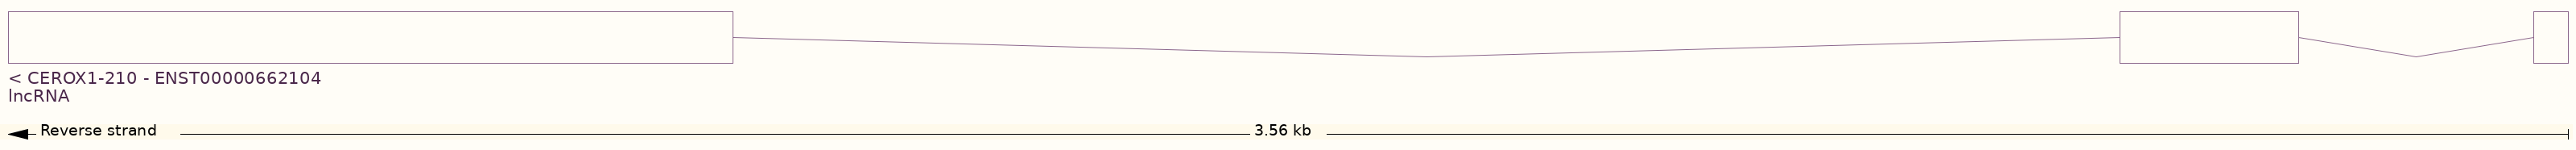
\includegraphics[width=\textwidth]{images/CEROX1-210.png}
    \caption{Diagrama del Transcrito.}
    \label{fig:CEROX1-210-diag}
\end{figure}

\begin{figure}[H]
    \centering
    \begin{minipage}[c]{0.45\textwidth}
        \centering
        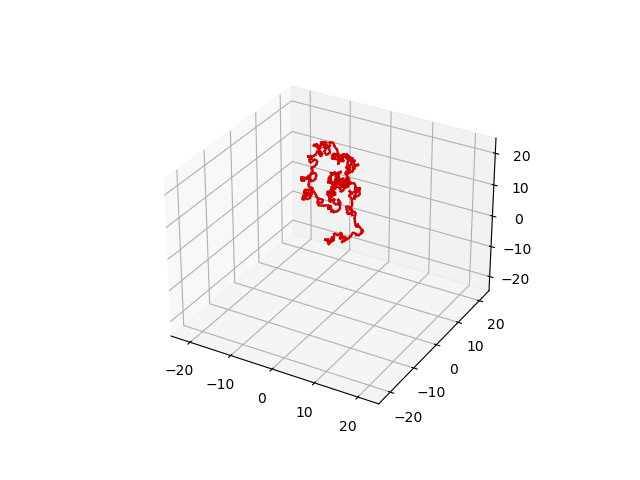
\includegraphics[width=\textwidth]{images/CEROX1-210-db_one.png}
        \caption{Conformación 3D CEROX1-210, una iteración.}
        \label{fig:CEROX1-210-one}
    \end{minipage}
    \hfill
    \begin{minipage}[c]{0.45\textwidth}
        \centering
        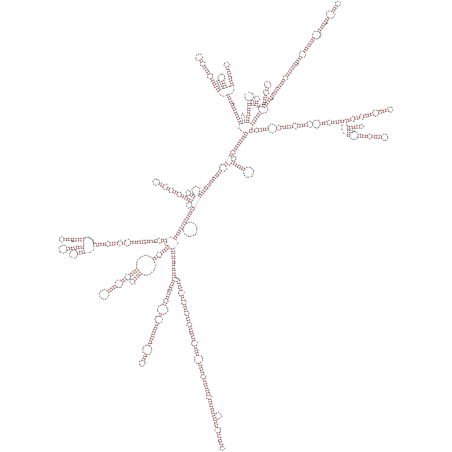
\includegraphics[width=\textwidth]{images/CEROX1-210-db_vrna.png}
        \caption{Conformación 2D CEROX1-210, ViennaRNA.}
        \label{fig:CEROX1-210-vrna}
    \end{minipage}
\end{figure}

\begin{figure}[H]
    \centering
    \begin{minipage}[c]{0.45\textwidth}
        \centering
        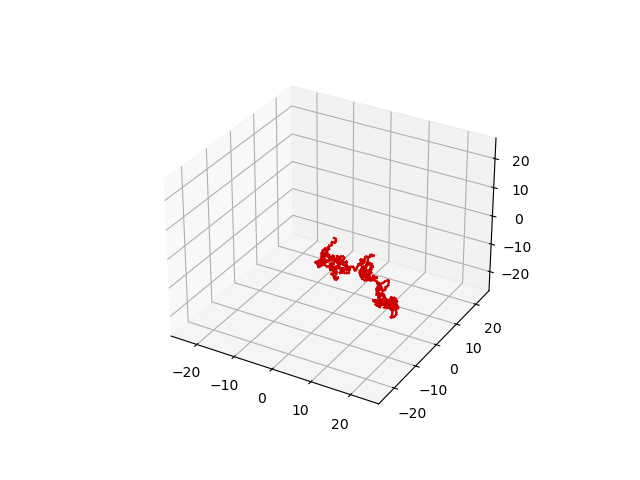
\includegraphics[width=\textwidth]{images/CEROX1-210-db_iter.png}
        \caption{Conformación 3D CEROX1-210, diez iteraciones.}
        \label{fig:CEROX1-210-multi}
    \end{minipage}
    \hfill
    \begin{minipage}[c]{0.45\textwidth}
        \centering
        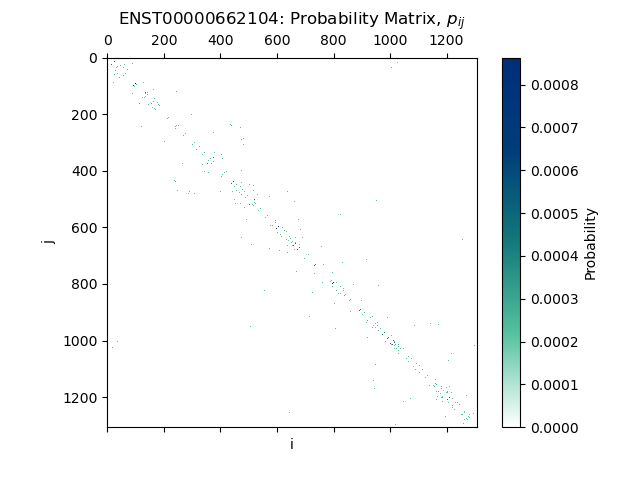
\includegraphics[width=\textwidth]{images/CEROX1-210-db_iter-matrix.png}
        \caption{Matriz de probabilidades, CEROX1-210.}
        \label{fig:CEROX1-210-matrix}
    \end{minipage}
\end{figure}



% ENST00000613346 yes
\newpage
\subsection*{PCDH15-221}\label{subsec:gene2}

\begin{figure}[H]
    \centering
    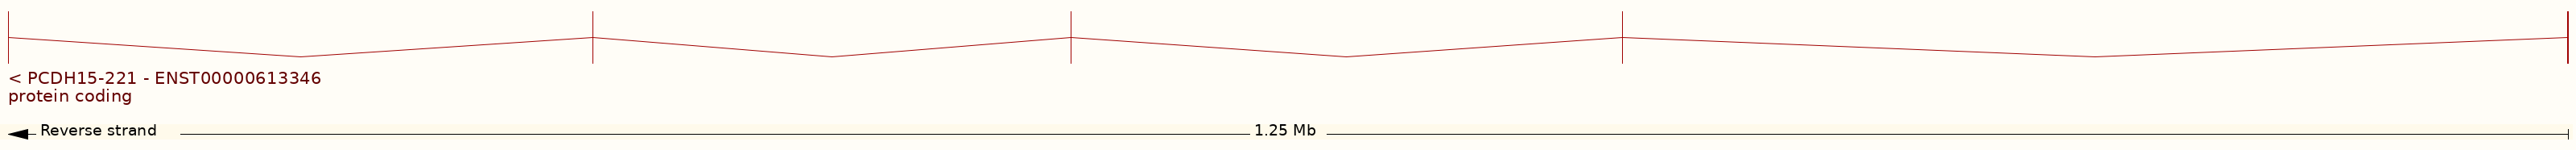
\includegraphics[width=\textwidth]{images/PCDH15-221.png}
    \caption{Diagrama del Transcrito.}
    \label{fig:PCDH15-221-diag}
\end{figure}

\begin{figure}[H]
    \centering
    \begin{minipage}[c]{0.31\textwidth}
        \centering
        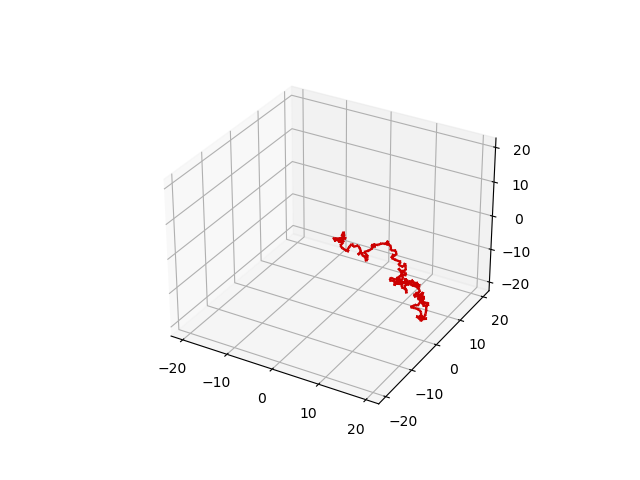
\includegraphics[width=\textwidth]{images/PCDH15-221-db_one.png}
        \caption{Conformación 3D PCDH15-221, una iteración.}
        \label{fig:PCDH15-221-one}
    \end{minipage}
    \hfill
    \begin{minipage}[c]{0.31\textwidth}
        \centering
        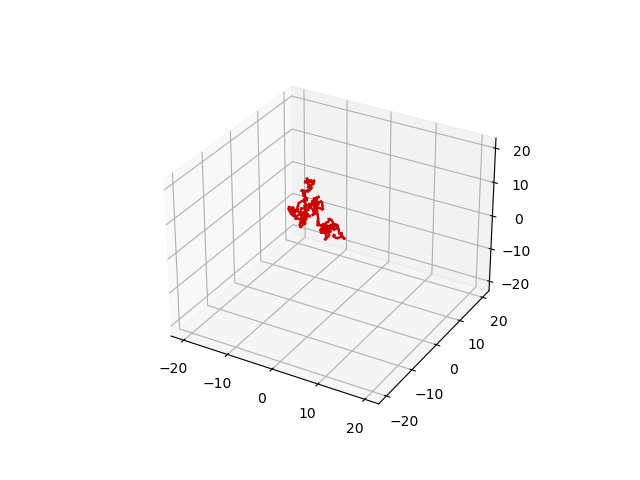
\includegraphics[width=\textwidth]{images/PCDH15-221-db_iter.png}
        \caption{Conformación 3D PCDH15-221, diez iteraciones.}
        \label{fig:PCDH15-221-multi}
    \end{minipage}
    \hfill
    \begin{minipage}[c]{0.31\textwidth}
        \centering
        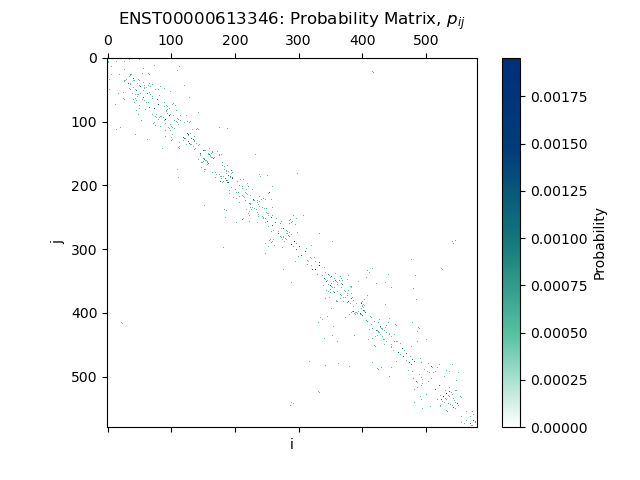
\includegraphics[width=\textwidth]{images/PCDH15-221-db_iter-matrix.png}
        \caption{Matriz de probabilidades, PCDH15-221.}
        \label{fig:PCDH15-221-matrix}
    \end{minipage}
\end{figure}

\begin{figure}[H]
    \centering
    \begin{minipage}[c]{0.45\textwidth}
        \centering
        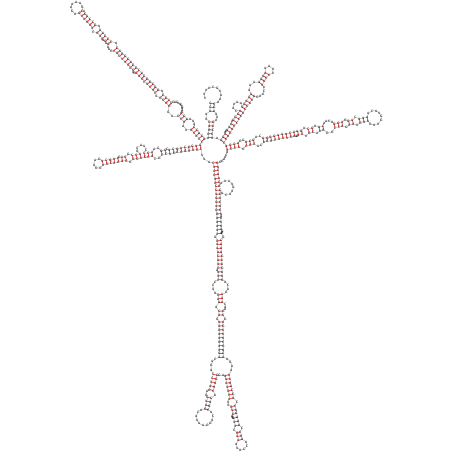
\includegraphics[width=\textwidth]{images/PCDH15-221-db_vrna.png}
        \caption{Conformación 2D PCDH15-221, ViennaRNA.}
        \label{fig:PCDH15-221-vrna}
    \end{minipage}
    \hfill
    \begin{minipage}[c]{0.45\textwidth}
        \centering
        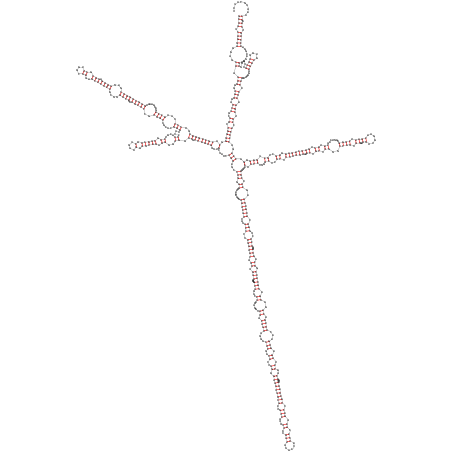
\includegraphics[width=\textwidth]{images/PCDH15-221-db_sqf.png}
        \caption{Conformación 2D PCDH15-221, SeqFold.}
        \label{fig:PCDH15-221-sqf}
    \end{minipage}
\end{figure}

% ENST00000575207 no
\newpage
\subsection*{VPS53-218}\label{subsec:gene3}

\begin{figure}[H]
    \centering
    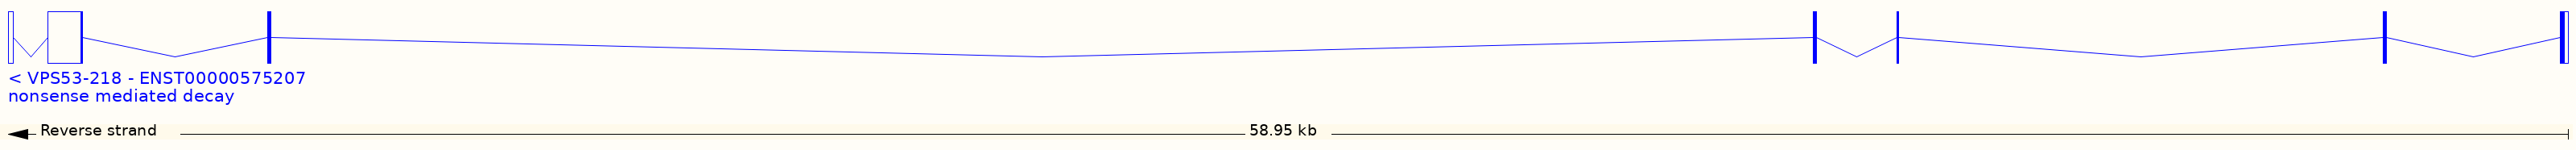
\includegraphics[width=\textwidth]{images/VPS53-218.png}
    \caption{Diagrama del Transcrito.}
    \label{fig:VPS53-218-diag}
\end{figure}

\begin{figure}[H]
    \centering
    \begin{minipage}[c]{0.45\textwidth}
        \centering
        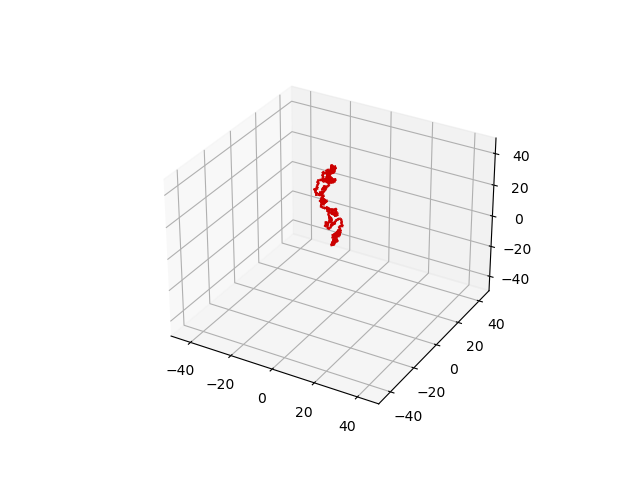
\includegraphics[width=\textwidth]{images/VPS53-218-db_one.png}
        \caption{Conformación 3D VPS53-218, una iteración.}
        \label{fig:VPS53-218-one}
    \end{minipage}
    \hfill
    \begin{minipage}[c]{0.45\textwidth}
        \centering
        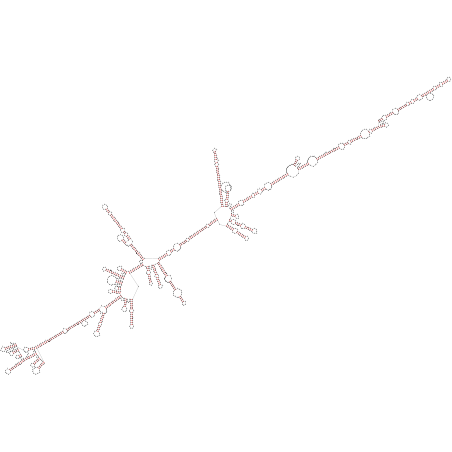
\includegraphics[width=\textwidth]{images/VPS53-218-db_vrna.png}
        \caption{Conformación 2D VPS53-218, ViennaRNA.}
        \label{fig:VPS53-218-vrna}
    \end{minipage}
\end{figure}

\begin{figure}[H]
    \centering
    \begin{minipage}[c]{0.45\textwidth}
        \centering
        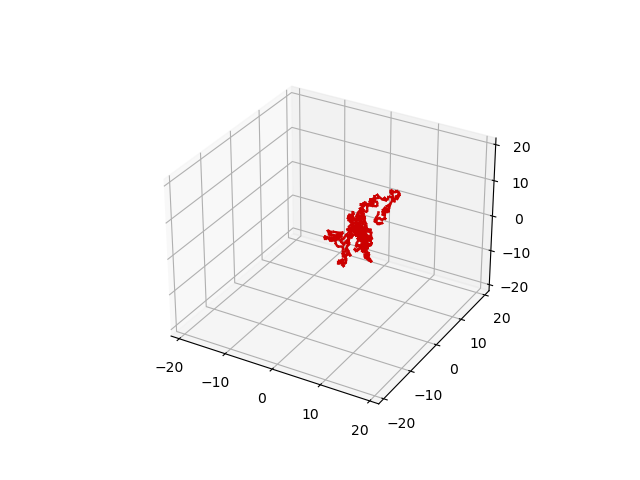
\includegraphics[width=\textwidth]{images/VPS53-218-db_iter.png}
        \caption{Conformación 3D VPS53-218, diez iteraciones.}
        \label{fig:VPS53-218-multi}
    \end{minipage}
    \hfill
    \begin{minipage}[c]{0.45\textwidth}
        \centering
        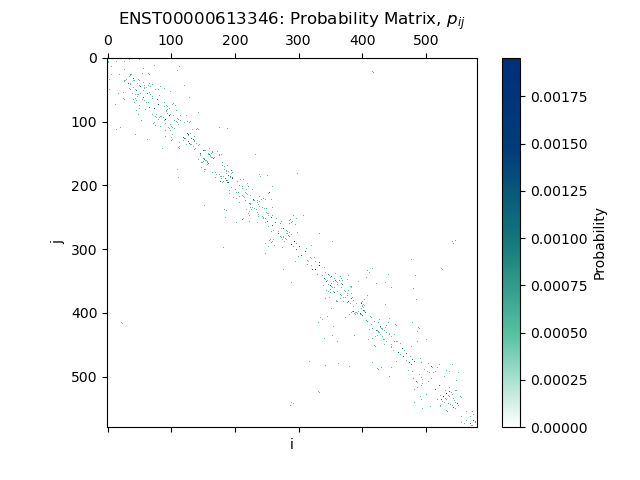
\includegraphics[width=\textwidth]{images/VPS53-218-db_iter-matrix.png}
        \caption{Matriz de probabilidades, VPS53-218.}
        \label{fig:VPS53-218-matrix}
    \end{minipage}
\end{figure}

% ENST00000506218 yes
\newpage
\subsection*{MACROH2A1-208}\label{subsec:gene4}

\begin{figure}[H]
    \centering
    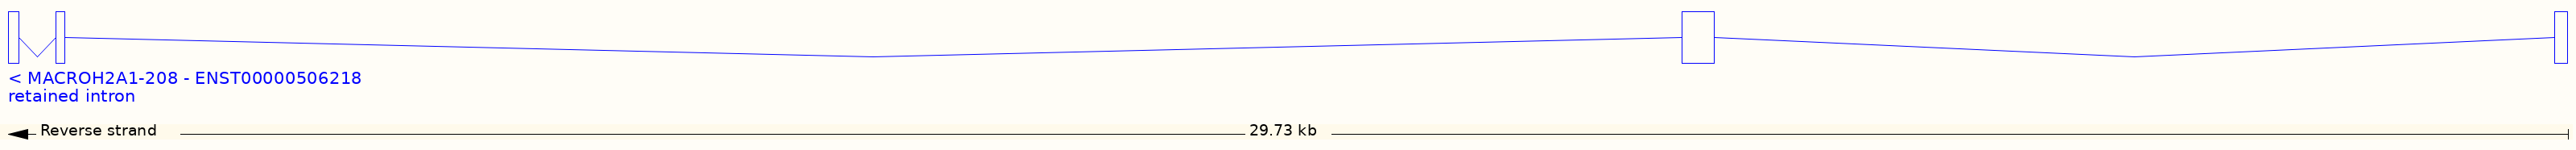
\includegraphics[width=\textwidth]{images/MACROH2A1-208.png}
    \caption{Diagrama del Transcrito.}
    \label{fig:MACROH2A1-208-diag}
\end{figure}

\begin{figure}[H]
    \centering
    \begin{minipage}[c]{0.31\textwidth}
        \centering
        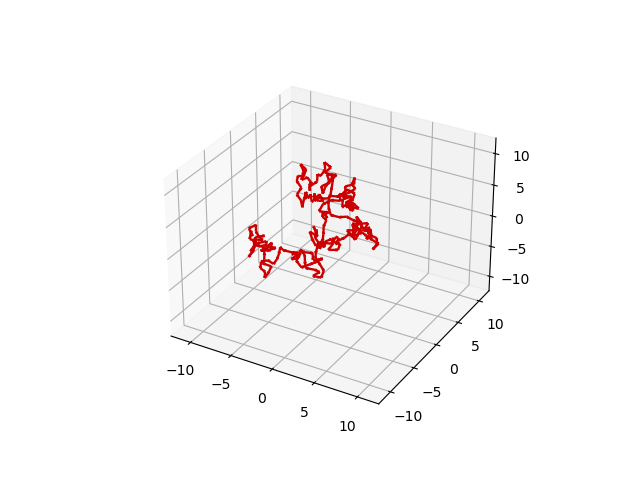
\includegraphics[width=\textwidth]{images/MACROH2A1-208-db_one.png}
        \caption{Conformación 3D MACROH2A1-208, una iteración.}
        \label{fig:MACROH2A1-208-one}
    \end{minipage}
    \hfill
    \begin{minipage}[c]{0.31\textwidth}
        \centering
        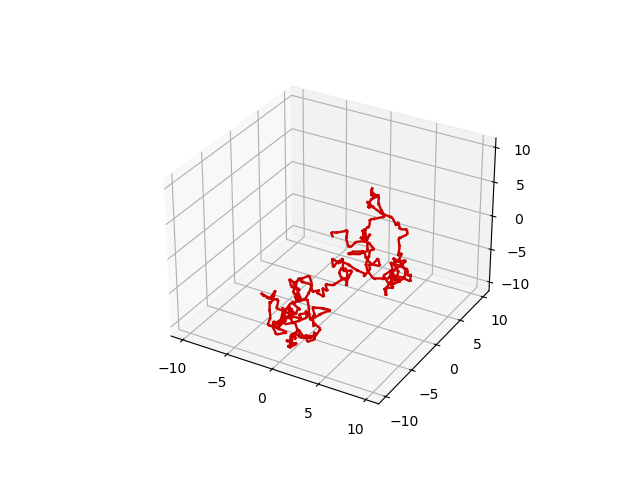
\includegraphics[width=\textwidth]{images/MACROH2A1-208-db_iter.png}
        \caption{Conformación 3D MACROH2A1-208, diez iteraciones.}
        \label{fig:MACROH2A1-208-multi}
    \end{minipage}
    \hfill
    \begin{minipage}[c]{0.31\textwidth}
        \centering
        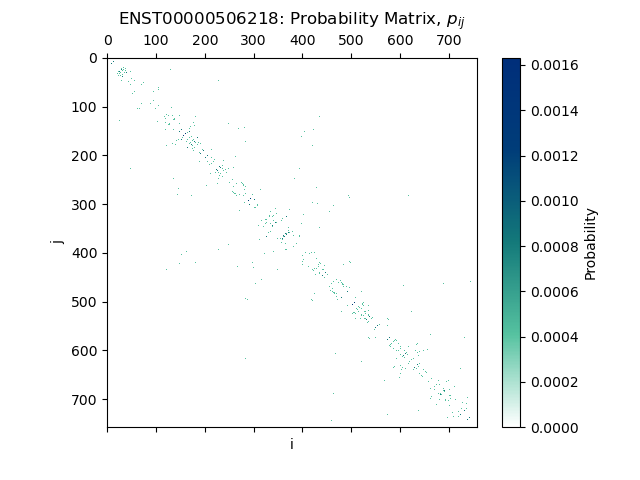
\includegraphics[width=\textwidth]{images/MACROH2A1-208-db_iter-matrix.png}
        \caption{Matriz de probabilidades, MACROH2A1-208.}
        \label{fig:MACROH2A1-208-matrix}
    \end{minipage}
\end{figure}

\begin{figure}[H]
    \centering
    \begin{minipage}[c]{0.45\textwidth}
        \centering
        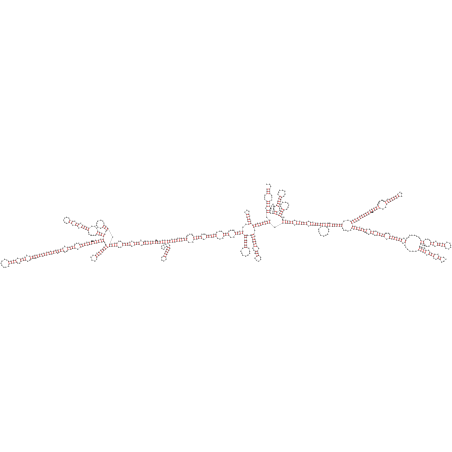
\includegraphics[width=\textwidth]{images/MACROH2A1-208-db_vrna.png}
        \caption{Conformación 2D MACROH2A1-208, ViennaRNA.}
        \label{fig:MACROH2A1-208-vrna}
    \end{minipage}
    \hfill
    \begin{minipage}[c]{0.45\textwidth}
        \centering
        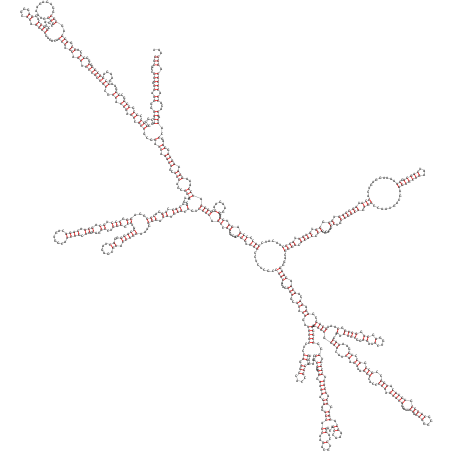
\includegraphics[width=\textwidth]{images/MACROH2A1-208-db_sqf.png}
        \caption{Conformación 2D MACROH2A1-208, SeqFold.}
        \label{fig:MACROH2A1-208-sqf}
    \end{minipage}
\end{figure}

% ENST00000217043 no
\newpage
\subsection*{R3HDML-201}\label{subsec:gene5}

\begin{figure}[H]
    \centering
    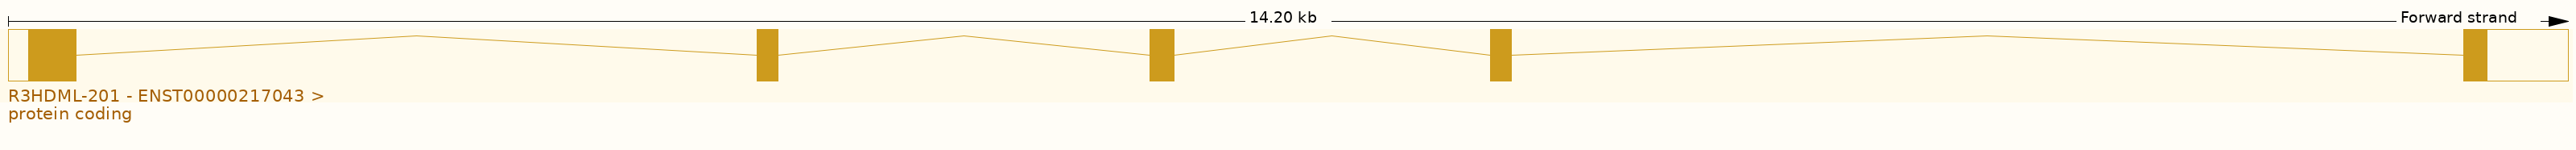
\includegraphics[width=\textwidth]{images/R3HDML-201.png}
    \caption{Diagrama del Transcrito.}
    \label{fig:R3HDML-201-diag}
\end{figure}

\begin{figure}[H]
    \centering
    \begin{minipage}[c]{0.45\textwidth}
        \centering
        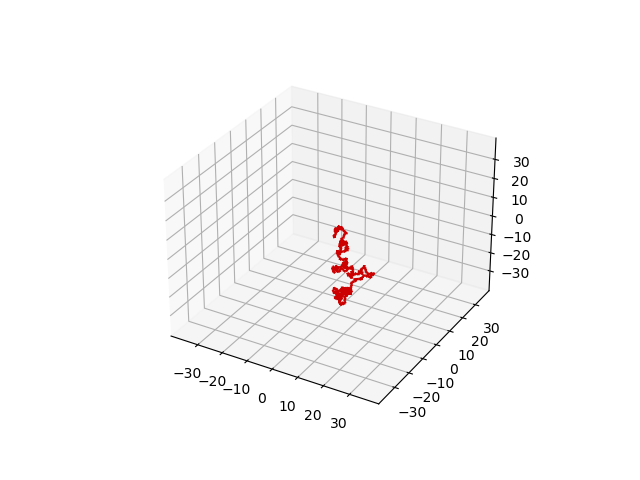
\includegraphics[width=\textwidth]{images/R3HDML-201-db_one.png}
        \caption{Conformación 3D R3HDML-201, una iteración.}
        \label{fig:R3HDML-201-one}
    \end{minipage}
    \hfill
    \begin{minipage}[c]{0.45\textwidth}
        \centering
        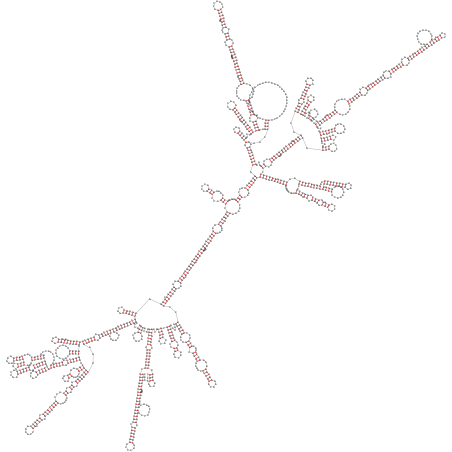
\includegraphics[width=\textwidth]{images/R3HDML-201-db_vrna.png}
        \caption{Conformación 2D R3HDML-201, ViennaRNA.}
        \label{fig:R3HDML-201-vrna}
    \end{minipage}
\end{figure}

\begin{figure}[H]
    \centering
    \begin{minipage}[c]{0.45\textwidth}
        \centering
        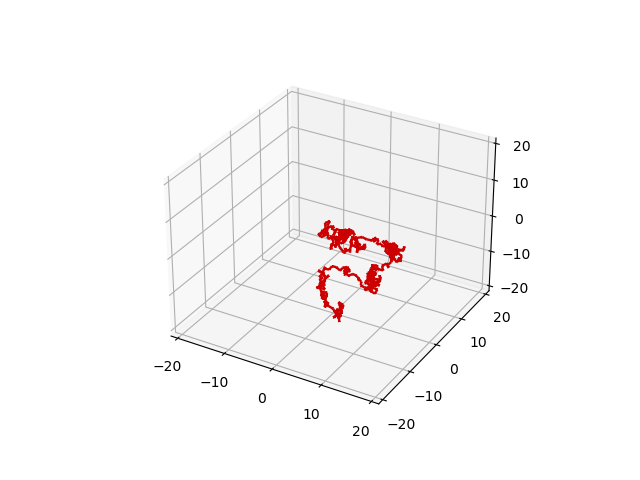
\includegraphics[width=\textwidth]{images/R3HDML-201-db_iter.png}
        \caption{Conformación 3D R3HDML-201, diez iteraciones.}
        \label{fig:R3HDML-201-multi}
    \end{minipage}
    \hfill
    \begin{minipage}[c]{0.45\textwidth}
        \centering
        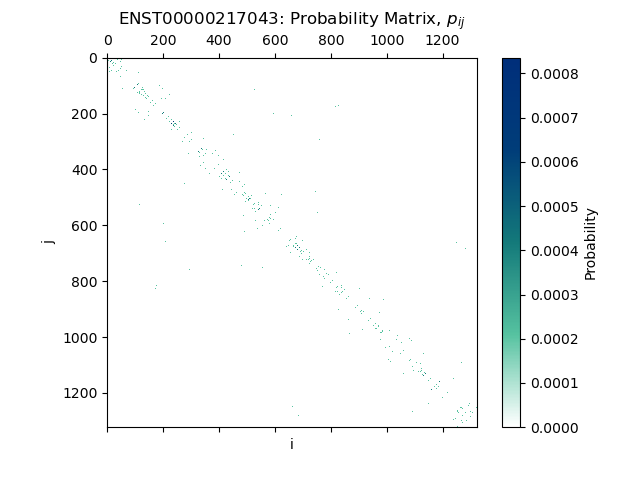
\includegraphics[width=\textwidth]{images/R3HDML-201-db_iter-matrix.png}
        \caption{Matriz de probabilidades, R3HDML-201.}
        \label{fig:R3HDML-201-matrix}
    \end{minipage}
\end{figure}

%\newpage
%\section{Apéndice II: Secuencias Dot Brackets}\label{sec:dot-brackets}

% ENST00000662104 no
%\normalsize\subsection*{CEROX1-210}\label{subsec:txtgene1}
%\footnotesize\verbatiminput{dot_brackets/dot_bracket-CEROX1-210.txt}

% ENST00000662104 no
%\newpage
%\normalsize\subsection*{PCDH15-221}\label{subsec:txtgene2}
%\footnotesize\verbatiminput{dot_brackets/dot_bracket-PCDH15-221.txt}

% ENST00000662104 no
%\newpage
%\normalsize\subsection*{VPS53-218}\label{subsec:txtgene3}
%\footnotesize\verbatiminput{dot_brackets/dot_bracket-VPS53-218.txt}

% ENST00000662104 no
%\newpage
%\normalsize\subsection*{MACROH2A1-208}\label{subsec:txtgene4}
%\footnotesize\verbatiminput{dot_brackets/dot_bracket-MACROH2A1-208.txt}

% ENST00000662104 no
%\newpage
%\normalsize\subsection*{R3HDML-201}\label{subsec:txtgene5}
%\footnotesize\verbatiminput{dot_brackets/dot_bracket-R3HDML-201.txt}

\end{document}